\chapter{Resultados de control de velocidad}
\label{cap: anexo control velocidad}

El presente apéndice muestra los resultados de los ensayos de validación de control de velocidad. El procedimiento de validación queda descrito en la sección \ref{sec: control velocidad ensayo}.

\section{Ejecución realizada con factor de escala de velocidad 10\%}

\begin{figure}[H]
    \centering
    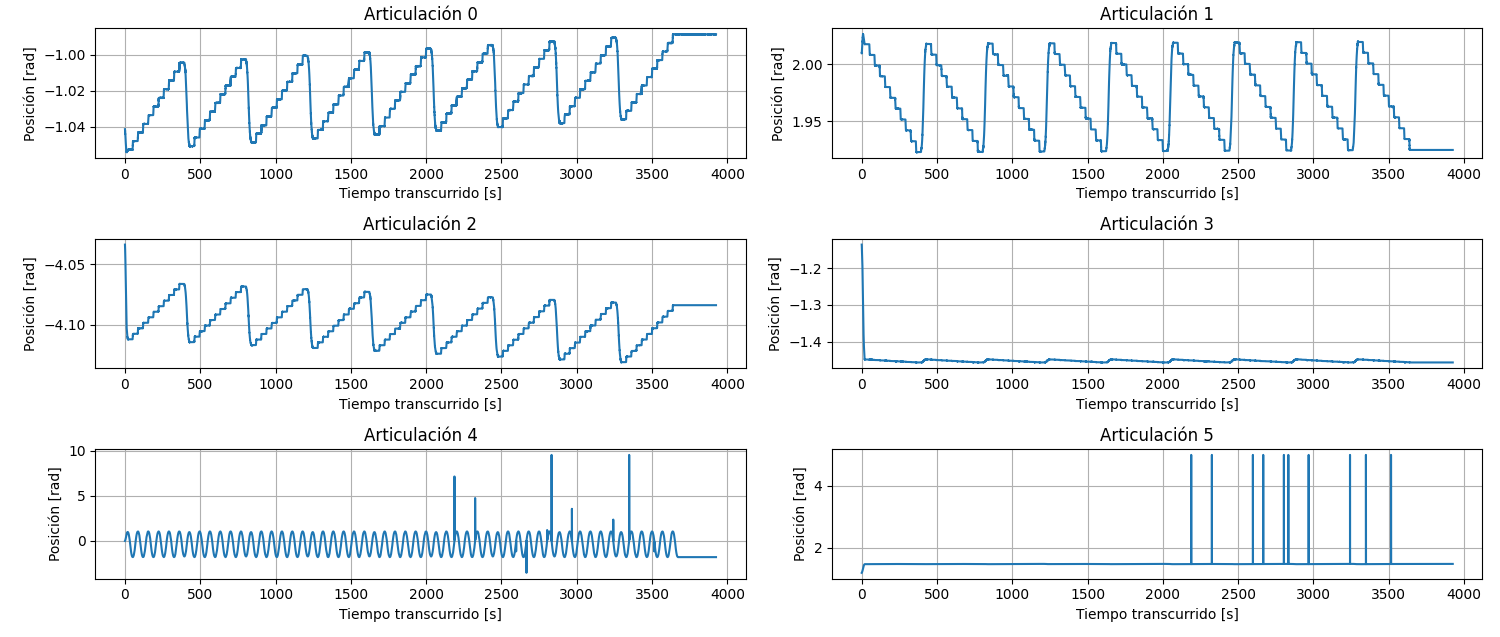
\includegraphics[scale=0.30]{figuras/ensayo_control_velocidad/posiciones articulares 0.1.png}
    \caption{Posiciones articulares. Factor 10\%}
    \label{fig:posiciones articulares 0.1}
\end{figure}

\begin{figure}[H]
    \centering
    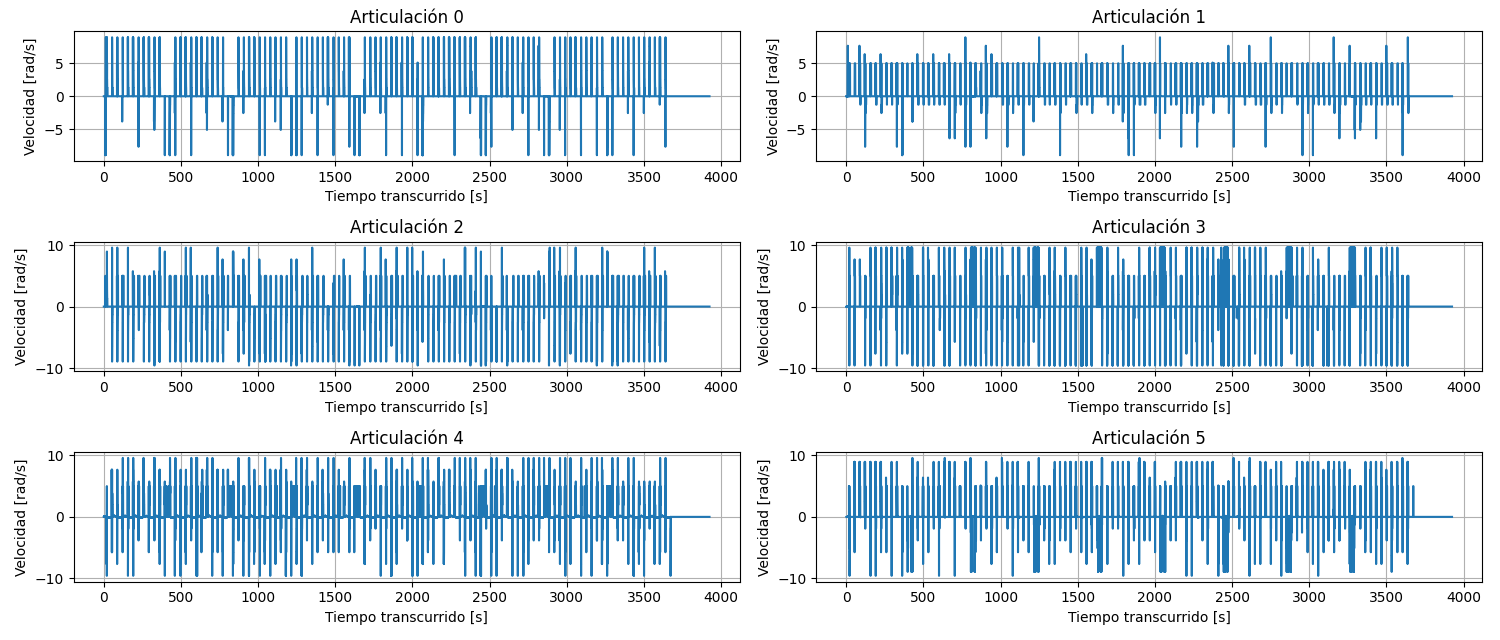
\includegraphics[scale=0.30]{figuras/ensayo_control_velocidad/velocidades articulares 0.1.png}
    \caption{Velocidades articulares. Factor 10\%}
    \label{fig:velocidades articulares 0.1}
\end{figure}

\begin{figure}[H]
    \centering
    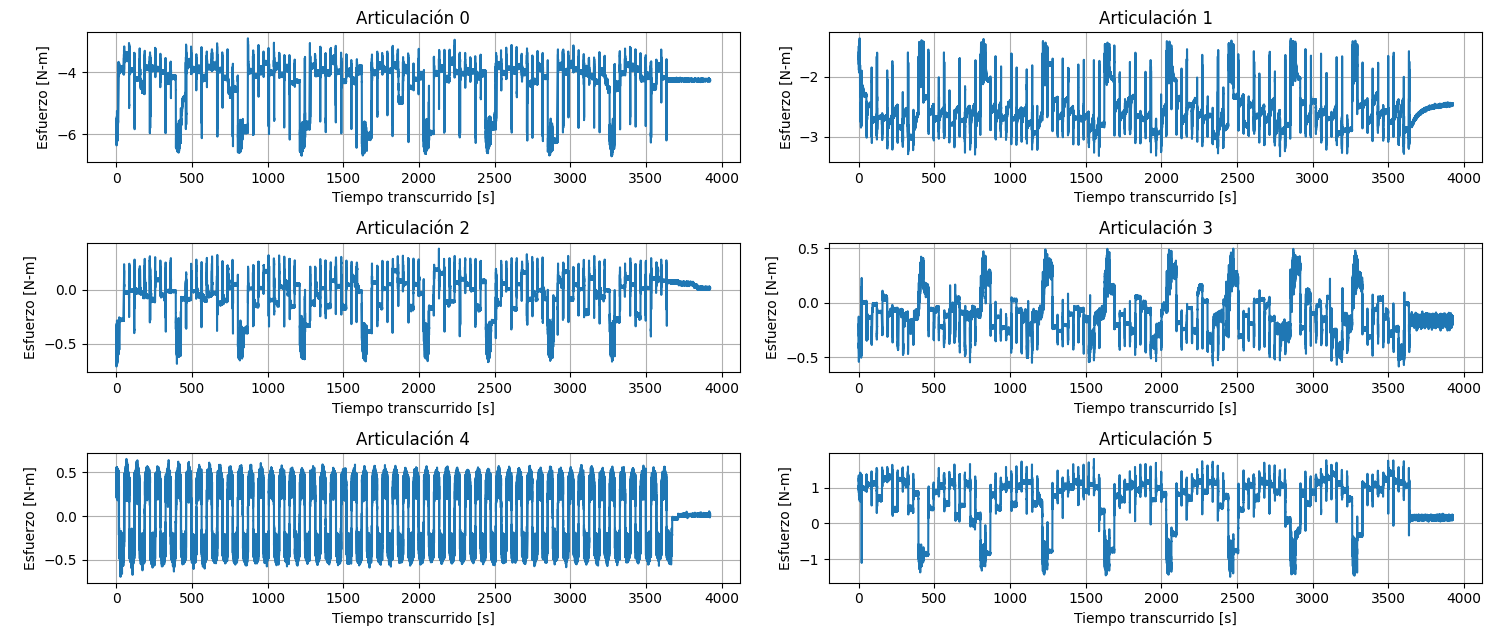
\includegraphics[scale=0.30]{figuras/ensayo_control_velocidad/esfuerzos 0.1.png}
    \caption{Esfuerzos articulares. Factor 10\%}
    \label{fig:esfuerzos articulares 0.1}
\end{figure}

\begin{figure}[H]
    \centering
    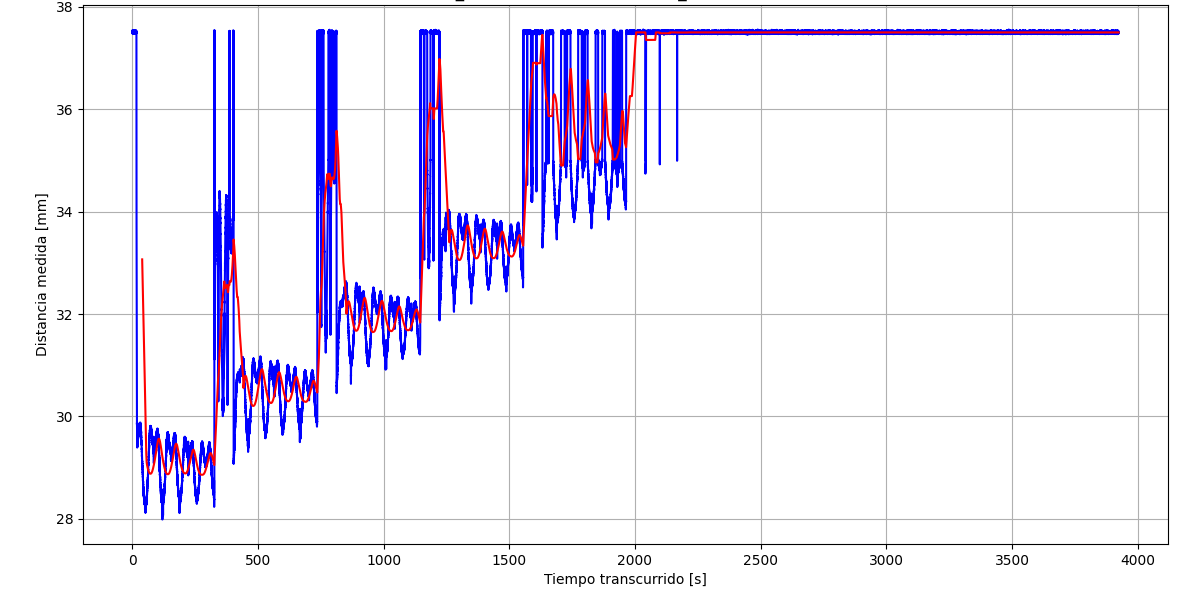
\includegraphics[scale=0.30]{figuras/ensayo_control_velocidad/laser 0.1.png}
    \caption{Distancia al sensor láseer. Factor 10\%}
    \label{fig:laser 0.1}
\end{figure}

\section{Ejecución realizada con factor de escala de velocidad 20\%}

\begin{figure}[H]
    \centering
    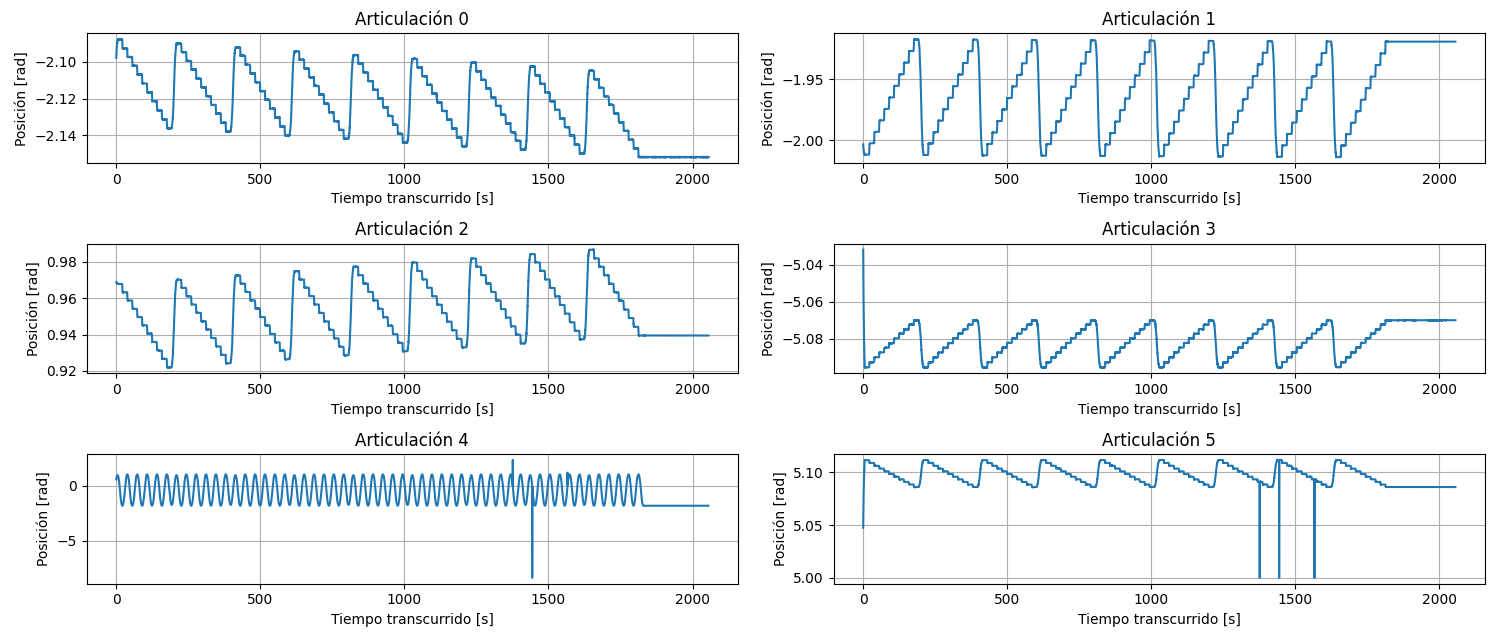
\includegraphics[scale=0.30]{figuras/ensayo_control_velocidad/posiciones articulares 0.2.png}
    \caption{Posiciones articulares. Factor 20\%}
    \label{fig:posiciones articulares 0.2}
\end{figure}

\begin{figure}[H]
    \centering
    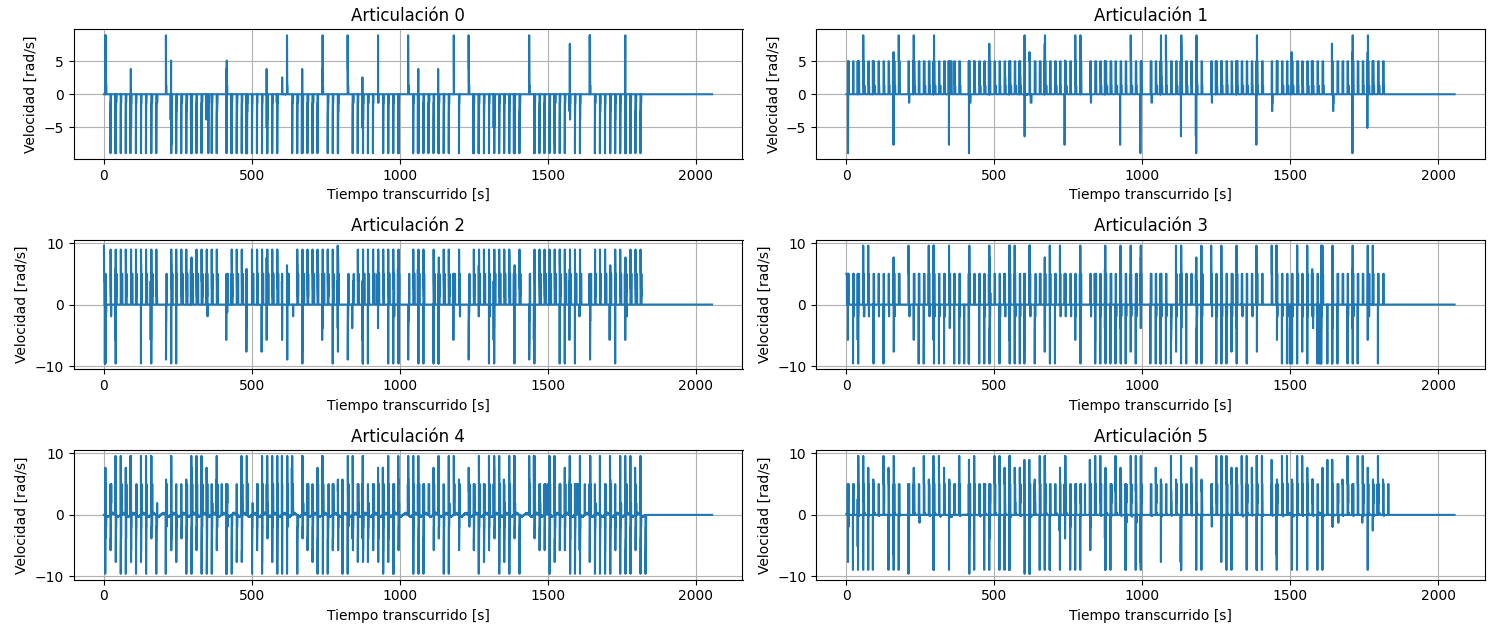
\includegraphics[scale=0.30]{figuras/ensayo_control_velocidad/velocidad articular 0.2.png}
    \caption{Velocidades articulares. Factor 20\%}
    \label{fig:velocidades articulares 0.2}
\end{figure}

\begin{figure}[H]
    \centering
    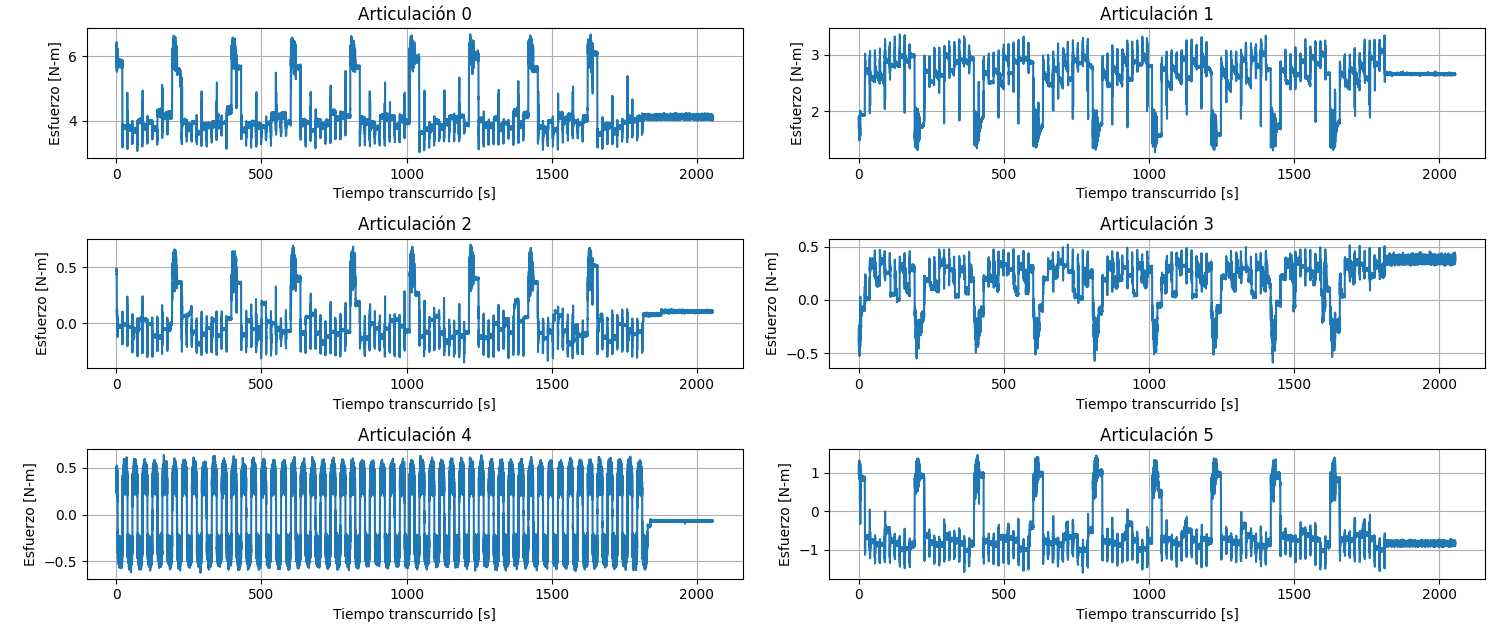
\includegraphics[scale=0.30]{figuras/ensayo_control_velocidad/esfuerzos 0.2.png}
    \caption{Esfuerzos articulares. Factor 20\%}
    \label{fig:esfuerzos articulares 0.2}
\end{figure}

\begin{figure}[H]
    \centering
    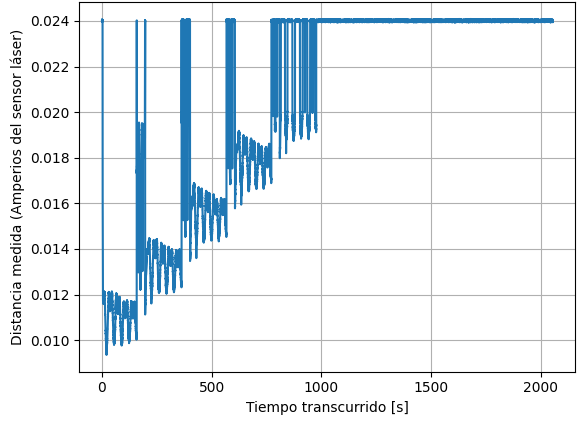
\includegraphics[scale=0.50]{figuras/ensayo_control_velocidad/laser 0.2.png}
    \caption{Distancia al sensor láser. Factor 20\%}
    \label{fig:laser 0.2}
\end{figure}

\section{Ejecución realizada con factor de escala de velocidad 40\%}

\begin{figure}[H]
    \centering
    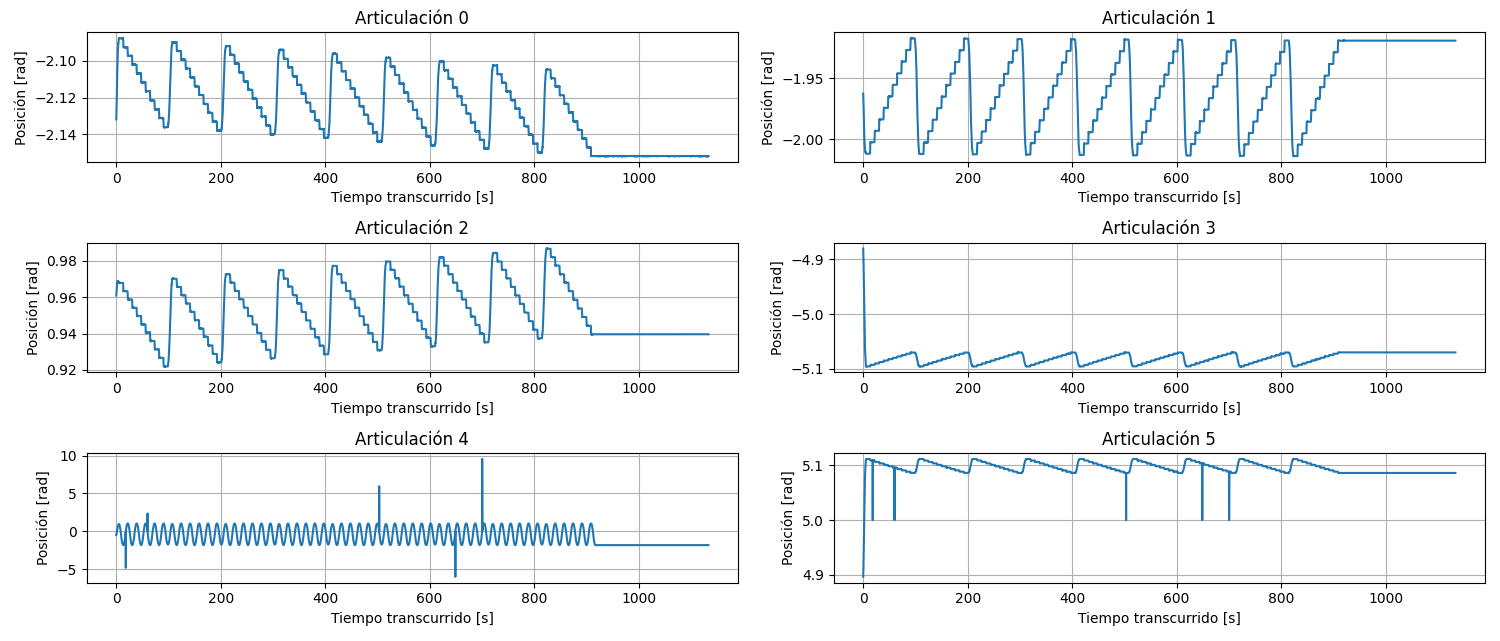
\includegraphics[scale=0.30]{figuras/ensayo_control_velocidad/posiciones articulares 0.4.png}
    \caption{Posiciones articulares. Factor 40\%}
    \label{fig:posiciones articulares 0.4}
\end{figure}

\begin{figure}[H]
    \centering
    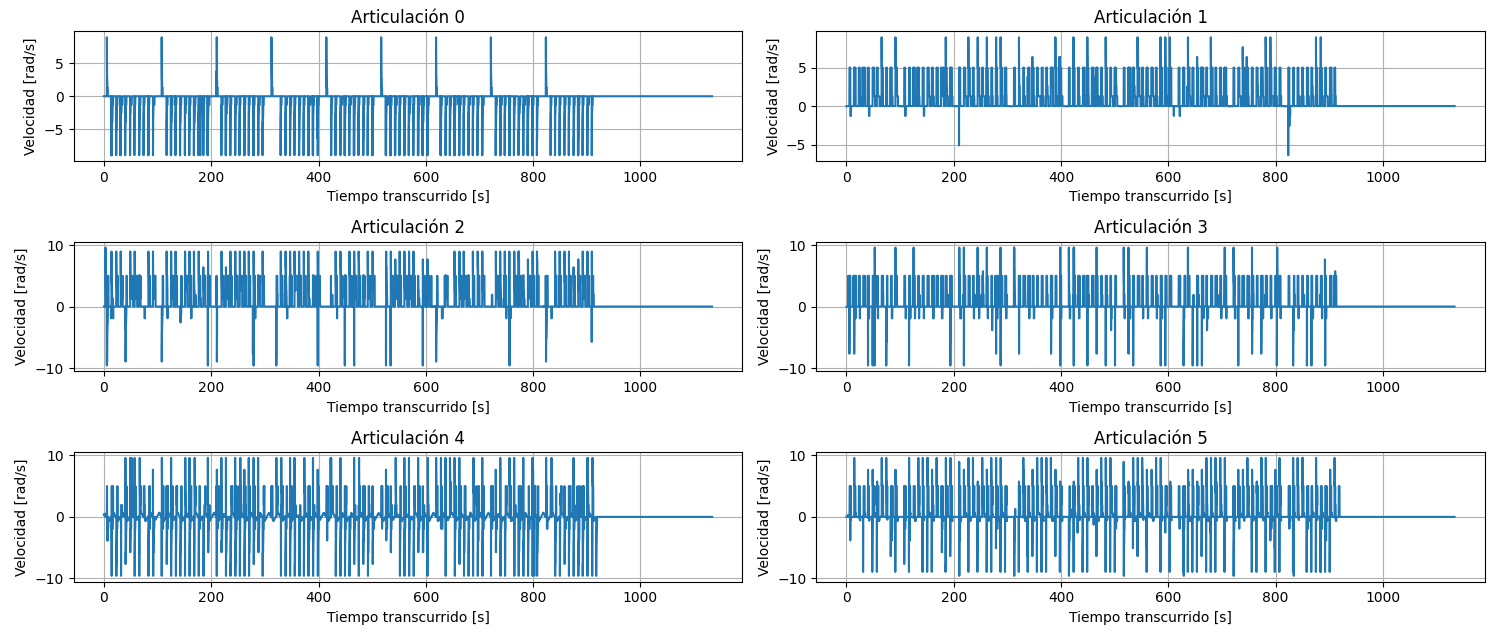
\includegraphics[scale=0.30]{figuras/ensayo_control_velocidad/velocidad articular 0.4.png}
    \caption{Velocidades articulares. Factor 40\%}
    \label{fig:velocidades articulares 0.4}
\end{figure}

\begin{figure}[H]
    \centering
    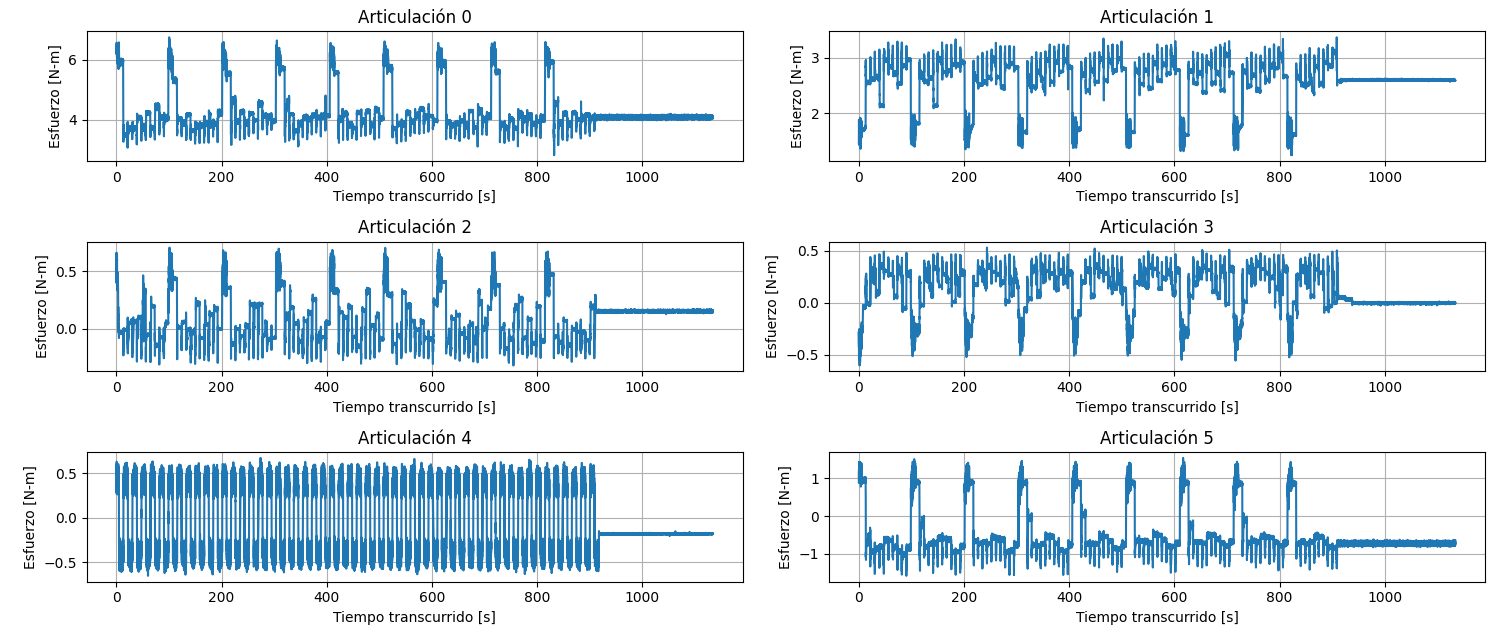
\includegraphics[scale=0.30]{figuras/ensayo_control_velocidad/esfuerzos 0.4.png}
    \caption{Esfuerzos articulares. Factor 40\%}
    \label{fig:esfuerzos articulares 0.4}
\end{figure}

\begin{figure}[H]
    \centering
    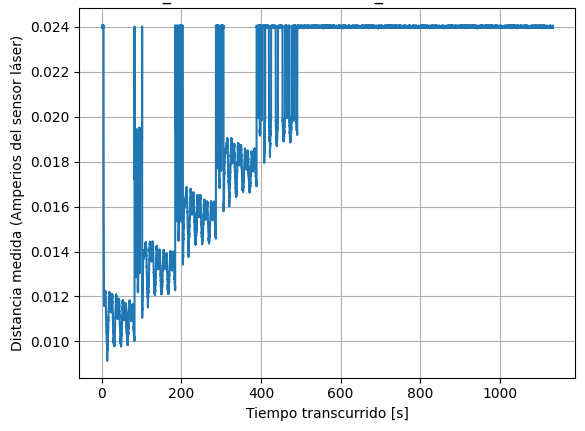
\includegraphics[scale=0.50]{figuras/ensayo_control_velocidad/laser 0.4.png}
    \caption{Distancia al sensor láser. Factor 40\%}
    \label{fig:laser 0.4}
\end{figure}

\section{Ejecución realizada con factor de escala de velocidad 60\%}

\begin{figure}[H]
    \centering
    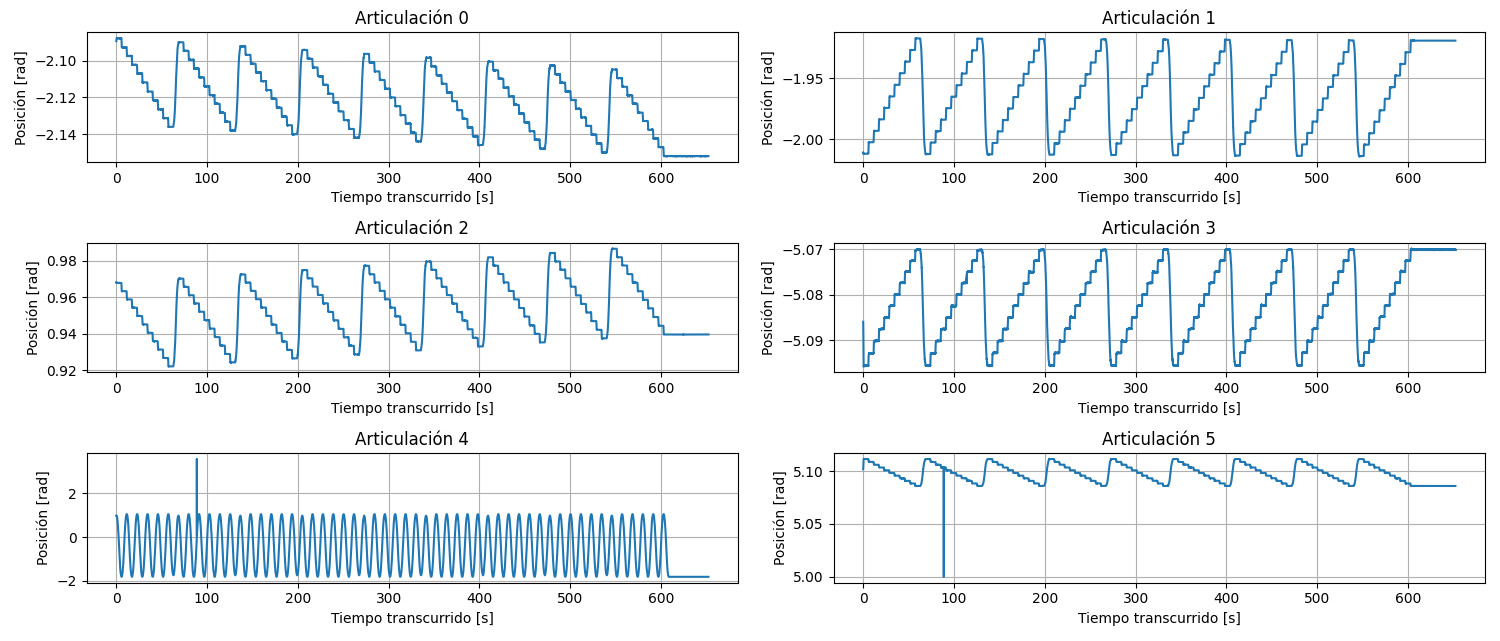
\includegraphics[scale=0.30]{figuras/ensayo_control_velocidad/posiciones articulares 0.6.png}
    \caption{Posiciones articulares. Factor 60\%}
    \label{fig:posiciones articulares 0.6}
\end{figure}

\begin{figure}[H]
    \centering
    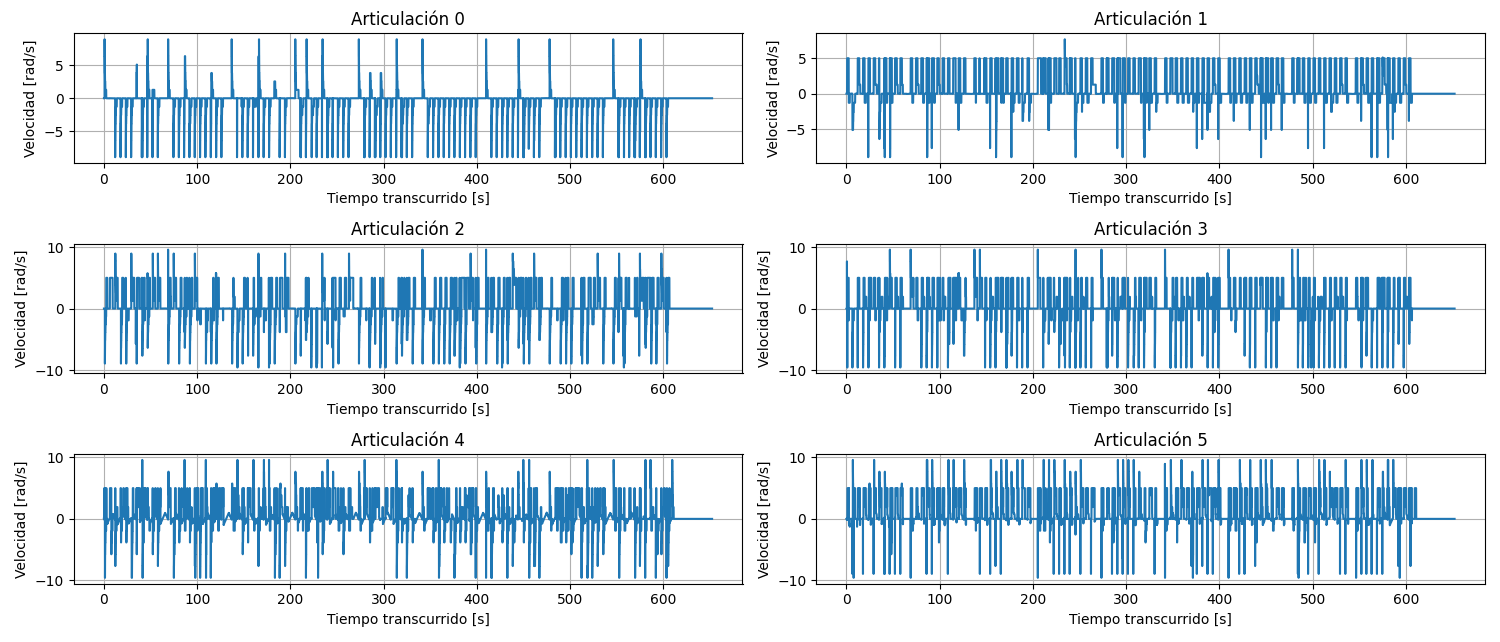
\includegraphics[scale=0.30]{figuras/ensayo_control_velocidad/velocidades articulares 0.6.png}
    \caption{Velocidades articulares. Factor 60\%}
    \label{fig:velocidades articulares 0.6}
\end{figure}

\begin{figure}[H]
    \centering
    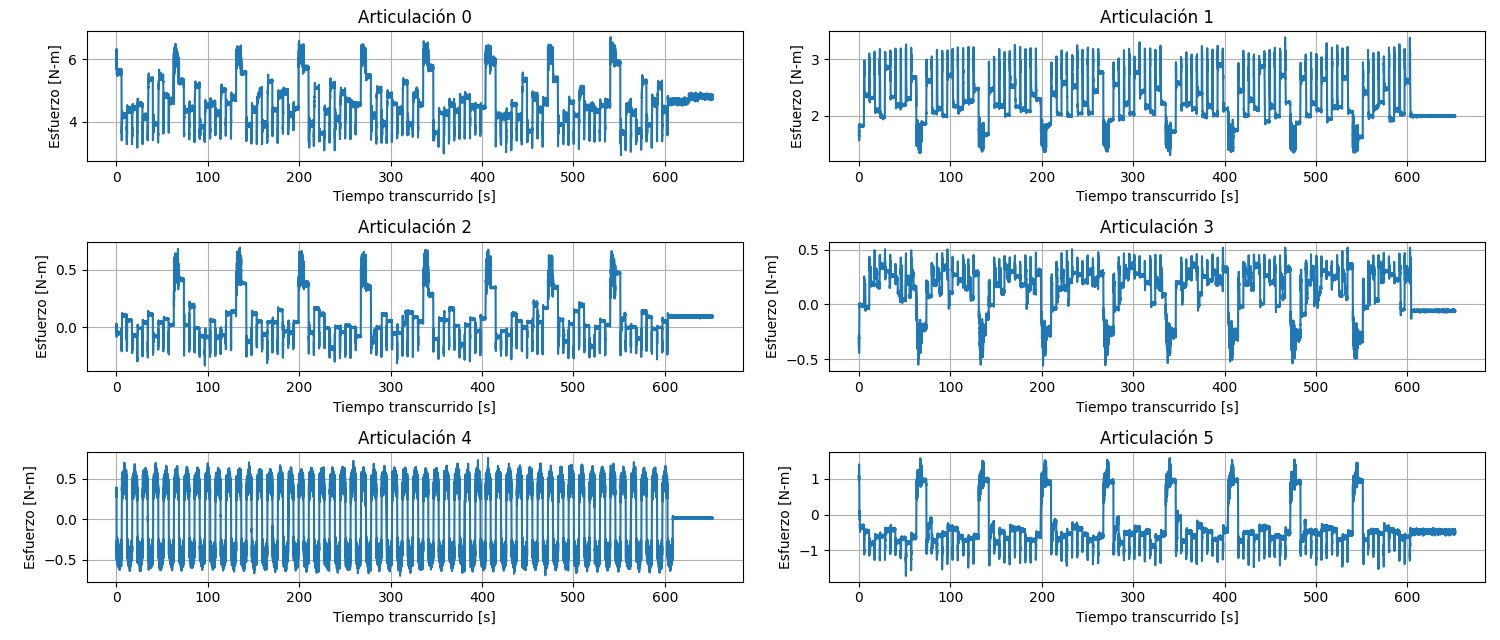
\includegraphics[scale=0.30]{figuras/ensayo_control_velocidad/esfuerzos articulares 0.6.png}
    \caption{Esfuerzos articulares. Factor 60\%}
    \label{fig:esfuerzos articulares 0.6}
\end{figure}

\begin{figure}[H]
    \centering
    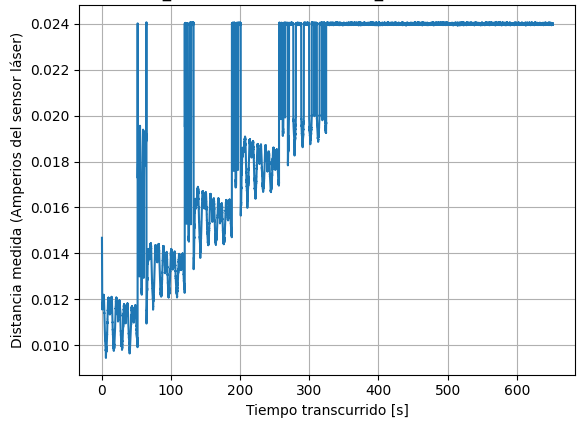
\includegraphics[scale=0.50]{figuras/ensayo_control_velocidad/laser 0.6.png}
    \caption{Distancia al sensor láser. Factor 60\%}
    \label{fig:laser 0.6}
\end{figure}
